\section{Including SVG in your project}
\label{svg}
The Makefile allows you to put svg files (e.g., drawn with an open source tools such as Inkscape) in the {\tt images } folder (or any subfolder).
The svg files are automatically watched and converted by the Makefile to get your paper always up to date.
If you don't like the {\tt images} folder, it can be changed in the Makefile, at the very beginning.

Here we include, in Figure~\ref{fig:gain}, an example graph. Followed by another one in Figure~\ref{fig:funky}.

{\bf Note:} the provide {\tt gitignore} file will prevent pdf files from being checked in the repository.
It uses a convention where if the pdf file name starts with ``pdf-'' then it is kept.
You might want to change that if you use a lot of pdf that are not generated by the Makefile.

\begin{figure}[t]
\begin{center}

\includegraphics[width=0.9\linewidth]{gain-of-learning-tools}
\end{center}
\caption{
  An amazing plot showing the importance of learning new things as the benefits are exponential :).
}
\label{fig:gain}
\end{figure}

\begin{figure}[t]
\begin{center}
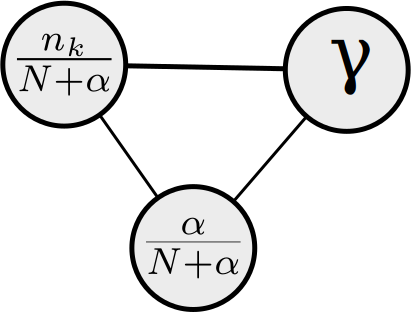
\includegraphics[width=0.45\linewidth]{subfolder/funky-graph}
and
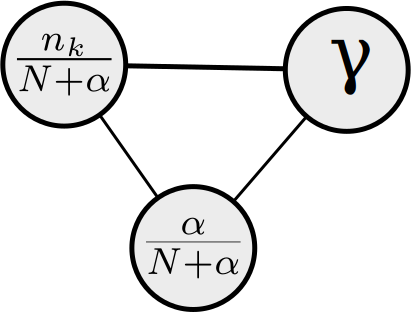
\includegraphics[width=0.45\linewidth]{subfolder/funky-graph}
\end{center}
\caption{
  Funky graph, twice, with math inside (used inkscape ``extension -- tex text'' and plain character for the $\gamma$).
}
\label{fig:funky}
\end{figure}

\section{Including EPS in your project}

Some libraries or tools cannot produce svg (nor pdf?) but can produce eps, format that pdflatex does not handle by default.
The Makefile allows for easy conversion of eps to pdf if needed.
An example of eps file is shown in Figure~\ref{fig:epsroc}.

\begin{figure*}[t]
\begin{center}
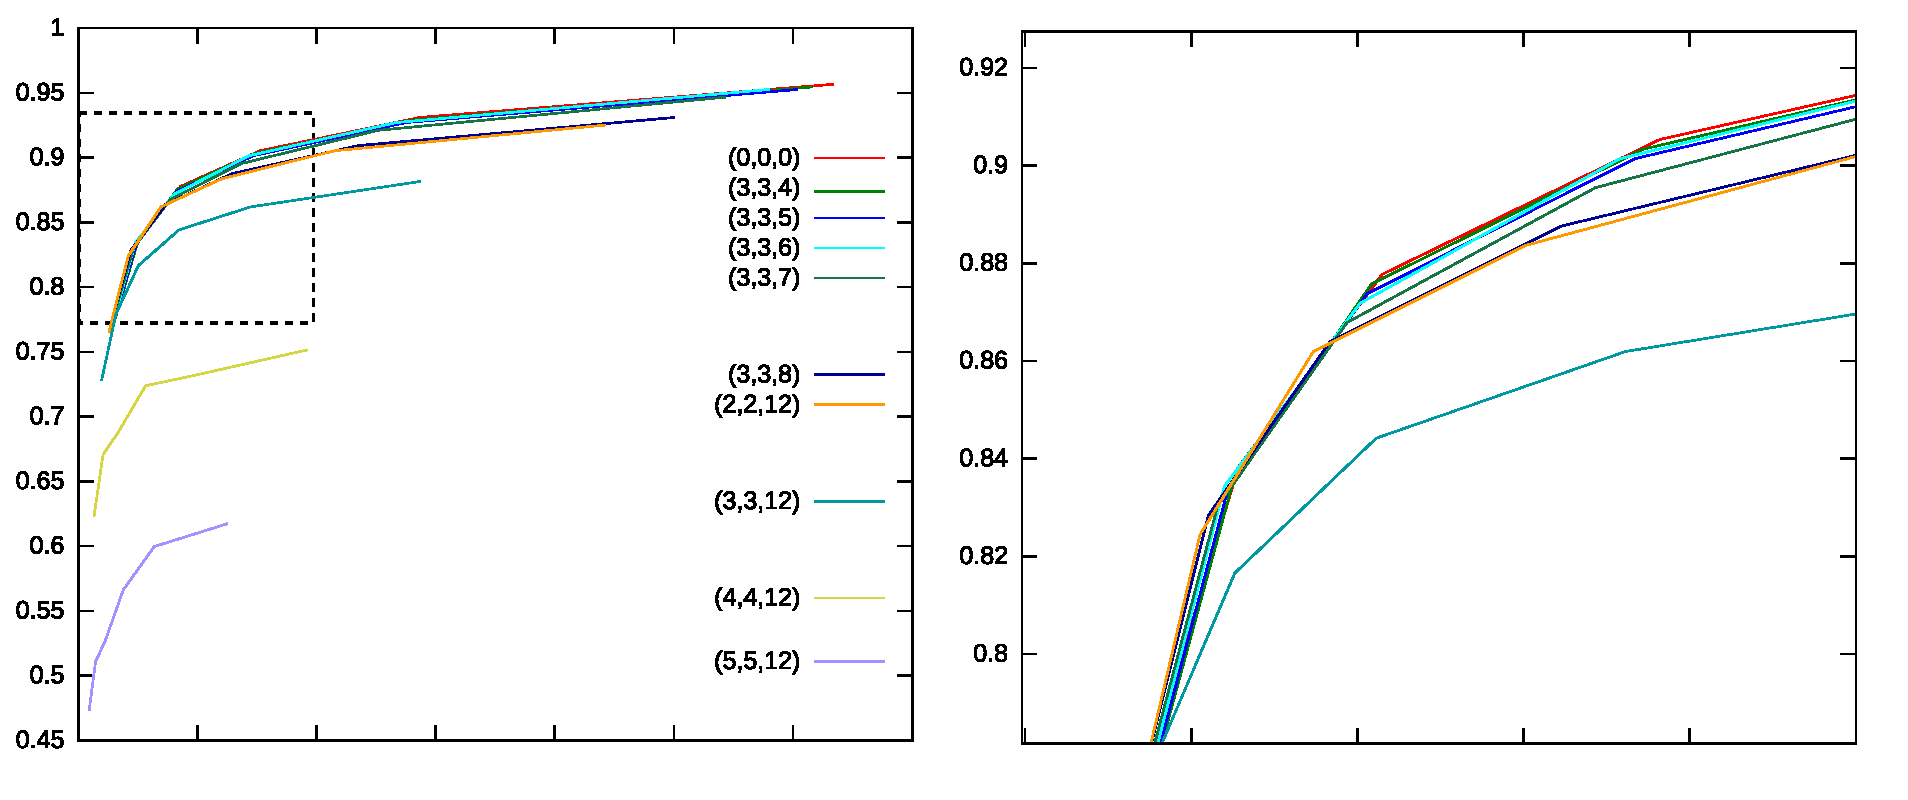
\includegraphics[width=0.9\linewidth]{subfolder/ROCs}
\end{center}
\caption{
  ROC curves of an amazing method for faster sliding window.
}
\label{fig:epsroc}
\end{figure*}


\section{wikipedia: Embodied Cognition}
\label{sec:embodiement}
In philosophy, the embodied mind thesis holds that the nature of the human mind is largely determined by the form of the human body.
Philosophers, psychologists, cognitive scientists, and artificial intelligence researchers who study embodied cognition and the embodied mind argue that all aspects of cognition are shaped by aspects of the body.
The aspects of cognition include high level mental constructs (such as concepts and categories) and human performance on various cognitive tasks (such as reasoning or judgement).
The aspects of the body include the motor system, the perceptual system, the body's interactions with the environment (situatedness) and the ontological assumptions about the world that are built into the body and the brain.

The embodied mind thesis is opposed to other theories of cognition such as cognitivism, computationalism, and Cartesian dualism.
The idea has roots in Kant and 20th century continental philosophy (such as Merleau-Ponty).
The modern version depends on insights drawn from recent research in psychology, linguistics, cognitive science, dynamical systems, artificial intelligence, robotics and neurobiology.

\section{wikipedia: Carl Rogers}
Carl Ransom Rogers (January 8, 1902 -- February 4, 1987) was an influential American psychologist and among the founders of the humanistic approach (or client-centered approach) to psychology.
Rogers is widely considered to be one of the founding fathers of psychotherapy research and was honored for his pioneering research with the Award for Distinguished Scientific Contributions by the American Psychological Association in 1956.

The person-centered approach, his own unique approach to understanding personality and human relationships, found wide application in various domains such as psychotherapy and counseling (client-centered therapy), education (student-centered learning), organizations, and other group settings.
For his professional work he was bestowed the Award for Distinguished Professional Contributions to Psychology by the APA in 1972.
Towards the end of his life Carl Rogers was nominated for the Nobel Peace Prize for his work with national intergroup conflict in South Africa and Northern Ireland.
In a study by Haggbloom et al. (2002) using six criteria such as citations and recognition, Rogers was found to be the sixth most eminent psychologist of the 20th century and second, among clinicians, only to Sigmund Freud.

\smallsection{Selected work}

Just one paper for bibtex illustration~\cite{rogers1967person}.

\section{Conclusions and future work}
\label{sec:concl}
All this is amazing!
% TODoooo: keep these lines, they are used to illustate the makefile
Is there something ToDo?

But also, a double spacing ~:
also like~ that.

It's all good and I will be notified if you use {\tt make continous}.

